% !TEX root = root.tex
\chapter{\label{chap:snase}The Role of Protein Unfolding on Mechanical Evolution of a Protein Layer During its Formation}
\chaptermark{Protein Unfolding}

\section{Introduction}

Previous work by our group on the microrheology of the protein $\beta$-lactoglobulin layers\cite{Lee2010} supports a picture of layer formation through a gelation process, where proteins associate through intermolecular disulfide bonds. In Chapter \ref{chap:lysozyme}, my work applied similar techniques to layers of lysozyme in an effort to understand better those aspects of the viscoelastic transition in protein layers that are universal and those that are system specific. The lysozyme study 

Lysozyme, $\beta$-lactoglobulin, and SNase are single-chain globular proteins that have been widely studied for decades. They are stable in bulk solution (i.e., they do not rapidly aggregate) but they readily adsorb to the air--water interface. For the SNase study in particular, we isolated the role of protein unfolding in evolution of the layer's mechanical response. We studied wild-type SNase---the protein as it is found in nature---and an engineered variant that shared almost the same chemical composition but had a completely disordered, unfolded structure.


Previous work on the mechanical properties of protein layers has characterized well-studied proteins like BSA, lysozyme, and $\beta$-lactoglobulin, surveying the evolution of surface pressure and interfacial viscosity during layer formation. While a variety of responses and layer evolutions are observed, it is difficult to conclude why differences are seen, how precisely the differences between these proteins� structure contribute to differences in the formation and the rheology of interfacial layers.

In this paper, we study the layer formation of two proteins that are nearly identical in composition but very different in structure. Specifically, we study SNase and engineered variant of SNase with only one residue changed. That one change catastrophically destabilizes the protein�s folded structure.


\begin{figure}
 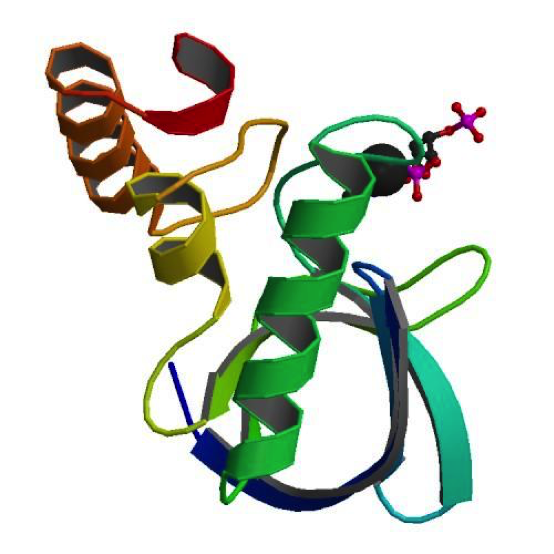
\includegraphics[width=\linewidth,keepaspectratio]{snase/ribbon-diagram}
 \caption[\lofimage{snase/ribbon-diagram}Ribbon diagram of Wild-Type SNase]{\label{fig:ribbon-diagram}This ribbon diagram shows the secondary structure of SNase. The $\alpha$-helix, positioned front and center from this perspective, acts a ``lid`` on the beta barrel (a beta sheet curved into a closed structure) beneath it. The interior of the beta barrel is hydrophobic, and the $\alpha$-helix helps keep water out. Change one residue in the middle of the helix creates a kink, effectively breaking the lid and ruining the stability of the folded structure.}
\end{figure}

\section{Experimental Methods}

\subsection{Protein Fabrication}

\subsubsection{PCR}

PCR is a standard, decades-old technique in biology, but a brief summary is included here for interested readers. 
Order a plasmid, a ring of DNA. Order a primer, a synthetic fragment of DNA chemically synthesized by joining base pairs, which largely compliments the plasmid but contains a snippet of noncomplemtary DNA. 

Put the primers and plasmids into a soup of loose ribonucleotides and DNA polymerase, which marches along the chain and builds a DNA polymer along complemtary strands. So, the original primers are extended to full strands, and then full copies are made as the process proceeds. This is PCR. It is a decades-old technique.

You subject the bacteria to thermal stress ("heat shock" up to about 40-50 C), and they imbibe the plasmids from the environment, looking for communally shared survival methods. Then the bacteria make the desired protein from the plasmids. Incidentally, synthesizing proteins without help from bacteria or cells is possible but challenging and expensive.

\subsection{Sample Preparation}



\subsection{Active Microrheology}

\section{Results}
\subsection{Wild-Type Layer Evolution}
\subsection{Disordered Layer Evolution}
\section{Discussion}
\section{Conclusion}